\chapter{Renewal Processes}
\textbf{Outset} We want to model replacement times of a machine. First we wait $T_1$ until we replace it, then we wait $T_2$ until replacing the replacement, and so on.

\noindent
\textbf{Questions:} After time $t$, how many replacements did we have to make ($N_t$)? What about the expected number $m(t)=\mathbb{E}_{} \left[ N_t \right] $?
What about the 'excess time', i.e. if we are at time $t$, how long until the next replacement ($E_t$, $e(t)=\mathbb{E}_{} \left[ E_t \right]$)? Or the age of the machine ($A_t$, $a(t)=\mathbb{E}_{} \left[ A_t \right] $).
{\color{blue} //I think we should elaborate on case 1 more, and leave out case 2, these correspond to the what we said in the lecture and not what is specifically in your notes, where you have multiple examples.//}

Case 1: $T_1, T_2, \ldots$  $Exp(\lambda)$ random variables: $m(t)=t\lambda$, $E_t$ also $Exp(\lambda)$, then $e(t)= \frac{1}{\lambda}$, $A_t$ is also $Exp(\lambda)$.

Case 2: More complicated.

\section{Definition and First Properties}
\textbf{Framework} $(\Omega, \mathcal{F}, \mathbb{P})$ Probability space, $T_1, T_2, \ldots $  i.i.d. random variables on $\mathbb{R}_+$ 'inter-arrival times', such that $\mathbb{P}_{} \left[ T_i = 0 \right] < 1$, $\mu = \mathbb{E}_{} \left[ T_1 \right] \in (0, \infty]$. $F(t) =  \mathbb{P}_{} \left[ T_1 \leq t \right] $, $S_n = \sum_{i=1}^{n} T_i,\ S_0 =0$ 'renewal times'.
\begin{defn}
	The continuous time stochastic process $(N_t)_{t\geq 0}$ defined by:
\begin{align}
	\forall t \geq 0: N_t = \sum_{k=1}^{\infty} \mathbbm{1}_{S_k \leq t}
\end{align}
is called the \emph{renewal process with arrival distribution $F$}.
\end{defn}
{\color{blue}
\begin{rmk}[]
	It is important to differentiate between continuous time and continuous stochastic processes. Continuous time stochastic process are defined for every $t \in \mathbb{R}$ and may include jumps, meanwhile continuous stochastic processes follow continuous trajectories (eg.  Brownian Motion) and are not the subject of this course.
\end{rmk}
}

\begin{ex}[]
	\begin{enumerate}
		\item $pp(\lambda ), \lambda> 0,\ T_i$ a $Exp(\lambda)$ random variable,
		\item $(T_i)_{i\geq 1}$ i.i.d. $Exp(\lambda)$, $(X_i)_{i\geq 1}$  i.i.d. $Ber(\frac{1}{2})$, $T_i'= X_i T_i$, where  $(T_i)$ and  $(X_i)$ are independent.
		\item 'Fat Tailed' $\mathbb{P}_{} \left[ T_{i} \geq t \right] = \frac{1}{\sqrt{1+t}} \mathbbm{1}_{t\geq 0}$
	\end{enumerate}
	
\end{ex}

{\color{blue}
\begin{defn}
	Let $N=(N_t)_{t \geq 0}$ be a continuous time stochastic process with values in $\mathbb{R}$. We say that $N$ is a \emph{counting process} if the following holds a.s.
\begin{enumerate}
	\item $N_0 = 0$ a.s.,
	\item  $t \mapsto N_t$ is non-decreasing, right continuous, with values in $\mathbb{N}$.
\end{enumerate}
\end{defn}
}

\begin{prop}[]
	$N = (N_t)_{t\geq 0}$ is a counting process \footnote{without the condition that $N_0=0$ a.s.} with jump times $S_1, S_2, \ldots $ and $\lim_{t \to \infty} N_t = + \infty$.
\end{prop}
{\color{blue} //Is there a reason to use $+\infty$ rather than just $\infty$?. Also we have not defined a counting process at this point in time, because we are doing renewal processes before PP.//}
\begin{proof}
	Since $\mathbb{P}_{} \left[ T_i>0 \right] >0$, there exists $\alpha > 0$ such that $\mathbb{P}_{} \left[  T_i \geq \alpha  \right] >0$. Indeed $\mathbb{P}_{} \left[ T_1 >0 \right]  = \mathbb{P}_{} \left[ \bigcup_{\alpha \in \mathbb{Q}_+} \{ T_i \geq \alpha\} \right] $. We have
	\begin{align}
		\sum_{i>0}^{} \mathbb{P}_{} \left[ T_i \geq \alpha  \right] = \infty.
	\end{align}
	Therefore, by {\color{blue} the} Borel-Cantelli lemma, $\mathbb{P}_{} \left[A\right] =1$. Where
	\begin{align}
	A=	\left\{\omega: T_i(\omega) \geq \alpha \textrm{ for infinitely many } i \right\}.
	\end{align}
	For every $\omega \in A$, $S_n(\omega) \stackrel{n \to \infty}{\to} \infty$, and therefore
	\begin{align}
		t \mapsto N_t(\omega) = \sum_{n> 0}^{} \mathbbm{1}_{S_n(\omega) \leq t} 
	\end{align}
is a non-decreasing function with values in $\mathbb{N}$.	
\end{proof}


\begin{prop}[]
	There exists $c> 0$ such that
	\begin{align}
		\forall t\geq 0\ \mathbb{E}_{} \left[ e^{cN_t} \right] \leq e^{\frac{1+t}{c}}
	\end{align}
\end{prop}
\begin{rmk}[]
	In particular, for every $t \geq 1$, we have 
	\begin{align}
		\mathbb{E}_{} \left[ e^{c \frac{N_t}{t}} \right] \stackrel{\textrm(Jensen)}{\leq} \mathbb{E}_{} \left[ e^{cN_t} \right]^{\frac{1}{t}} \leq e^{\frac{2}{c}}	
	\end{align}
and
\begin{align}
	\mathbb{E}_{} \left[ \left( \frac{N_t}{t}\right)^d \right] \leq \frac{k!}{c^k}e^{\frac{2}{c}}.
\end{align}
\end{rmk}
\begin{proof}
	As before, we can pick $\alpha>0$ such that $\mathbb{P}_{} \left[ T_1 \geq \alpha  \right] >0$. For every $i> 0$, define
	\begin{align}
		T_i' = \alpha \mathbbm{1}_{T_i \geq \alpha}. 
	\end{align}
	We have $T_i' \leq T_i$ a.s. and $(T_i')$ are i.i.d. random variables with 
	\begin{align}
		T_i' = 
		\begin{cases}
			\alpha & \textrm{with probability } \beta \\
			0 & \textrm{with probability } 1-\beta
		\end{cases}
	\end{align}
	where $\beta = \mathbb{P}_{} \left[ T_1 \geq \alpha \right] > 0 $. Define $S_n'= \sum_{i=1}^{n} T_i'$ and the renewal process
	\begin{align}
		N_t' = \sum_{n> 0}^{} \mathbbm{1}_{S_n' \leq t} .
	\end{align}
	As in example {\color{blue} this example isn't here yet}, we have that
	\begin{align}
		N_t' = \stackrel{\textrm{(law)}}{=} X_0 + \sum_{i=1}^{\lfloor \frac{t}{\alpha } \rfloor} (1 + X_i),
	\end{align}
	where $(X_i)$ are geometric random variables with success parameter $\beta$. Therefore, for $c> 0$ such that $(1-\beta)e^c<1$, we have for all $t\geq 0$
	\begin{align}
	\mathbb{E}_{} \left[ e^{cN_t'} \right]  &= e ^{c\lfloor \frac{t}{\alpha}\rfloor} \prod_{i=0}^{\lfloor \frac{t}{\alpha }\rfloor} \mathbb{E}_{} \left[ e^{cX_i} \right] \\
						&\leq e^{\frac{ct}{\alpha }} \left( \frac{\beta }{1 - (1-\beta )e^c} \right)^{1 + \frac{t}{\alpha }} \\
						&\leq \left[ \left( \frac{e^c}{1 - (1-\beta )e^c} \right)^{\frac{1}{\alpha }} \right]^{1+t} \\
						&\leq e^\frac{1+t}{c}
	\end{align}
	for $c$ small enough (independent of $t$ ).
	{\color{blue} To get the second inequality, choose $\alpha \leq 1$ and use that $1+ \frac{t}{\alpha } \leq \frac{1+t}{\alpha }$ with this condition. This choice of $\alpha $ is justified as we are finding an upper bound, and $\alpha $ only appears in the denominators, thus we can choose it as small as needed.}	
\end{proof}


\begin{theorem}[Law of Large Numbers]
Write $\mu = \mathbb{E}_{} \left[ T_1 \right] $, then we have 
\begin{align}
	\lim_{t \to \infty} \frac{N_t}{t} = \frac{1}{\mu} \textrm{ a.s.}
\end{align}
\end{theorem}
\begin{rmk}[]
	If $\mu = \infty $, then $\lim_{t\to \infty } \frac{N_t}{t} = 0$ a.s.
\end{rmk}
\begin{proof}
	{\color{blue} // In your notes, you have $1/\mu $ and $\mu $ mixed up, I have made the correction here without putting it in blue, as I believe we spoke about this in the exercise class. //}

\textbf{Case 1:} $\mu < \infty $.
By the strong law of large numbers, we have 
\begin{align}
	\lim_{n \to \infty} \frac{S_{n+1}}{n+1} = \lim_{n \to \infty }\frac{S_n}{n+1} = \mu \textrm{ a.s.}
\end{align}
Notice that for every $t$ 
\begin{align}
	S_{N_t} \leq t \leq S_{N_{t}+1}.
\end{align}
Therefore,
\begin{align}
\underbrace{\frac{S_{N_t}}{N_t + 1}}_{\to \mu}
	\leq \frac{t}{N_t + 1} 
< \underbrace{\frac{S_{N_t + 1}}{N_t + 1}}_{\to \mu }.
\end{align}
Where the convergences are almost sure. Therefore $\lim_{t\to \infty } \frac{1 + N_t}{t} = \frac{1}{\mu }$ a.s., which implies that $\lim_{t \to \infty } \frac{N_t}{t} = \frac{1}{\mu} $ a.s.

\textbf{Case 2:} $\mu = \infty $.
Define $T_{i}^{(k)} = \min(k, T_i)$ for $k\geq 1$. This way we have $T_i^{(k)} \leq T_i$ a.s. and $T_i^{(k)} \uparrow T_i$ as $k \to \infty $ a.s. Consider the renewal process $N_t^{(k)}$ associated to the times $(T_i^{(k)})_{i\geq 1}$. Since $\mathbb{E}_{} \left[ T_i^{(k)} \right] \leq k < \infty$, we can apply case 1 to obtain that
\begin{align}
	\forall k \quad \lim_{t\to \infty }\frac{N_t^{(k)}}{t} = \frac{1}{\mathbb{E}_{} \left[ T_1^{(k)} \right] } \textrm{ a.s.}
\end{align}
Since $T_{i}^{(k)}\leq T_i$ a.s., we have $N_{t}^{(k)}\geq N_t$ a.s. Hence,
\begin{align}
	\forall k \quad \frac{1}{\mathbb{E}_{} \left[ T_1^{(k)} \right] } \geq \limsup_{t\to\infty} \frac{N_t}{t} \textrm{ a.s.}
\end{align}
Now, by monotone convergence, we have 
\begin{align}
	\lim_{k\to \infty } \mathbb{E}_{} \left[ T_1^{(k)} \right]  = \mathbb{E}_{} \left[ T_1 \right] = \infty,
\end{align}
and the two equations above conclude the proof.
\end{proof}

\begin{theorem}[Central Limit Theorem]
	Assume that $\mathbb{E}_{} \left[ T_1^2 \right] < \infty $. Write $\mu = \mathbb{E}_{} \left[ T_1 \right], \ \sigma^2 = Var(T_1)$. Then, assuming $\sigma>0$, we have
	\begin{align}
	\frac{N_t - \frac{t}{\mu }}{\sigma \sqrt{\frac{t}{\mu^3}}} \overset{\textrm{(law)}}{\underset{t \to \infty }{\longrightarrow}} \mathcal{N}(0,1)
	\end{align}
\end{theorem}
{\color{blue} // Proof not in notes, I believe this was an exercise, I could include that.//}

\begin{ex}[Renewal Reward Process]
	Let $(D_i)_{i\geq 1}$ be i.i.d. random variables with $D_i\geq 0$ and $\mathbb{E}_{} \left[ D_i \right] < \infty $. Define for every $t$ 
	\begin{align}
		R_t = \sum_{i\geq 1}^{} D_i \mathbbm{1}_{S_i \leq t}. 
	\end{align}
We call this the reward process, and $D_i$ the reward at time $S_i$. Then for $t $ large
\begin{align}
	\frac{R_t}{t}= \underbrace{\frac{1}{N_t} \sum_{i=1}^{N_t} D_i}_{\stackrel{\textrm{(LLN)}}{\to} \mathbb{E}_{} \left[ D_1 \right]} \underbrace{\frac{N_t}{t}}_{\to\frac{1}{\mu }}.
\end{align}
Therefore, $\frac{R_t}{t} \to \frac{\mathbb{E}_{} \left[ D_1 \right] }{\mu }$ a.s.
\end{ex}


\section{Renewal Function}
\begin{defn}
	The renewal function is defined by 
	\begin{align}
		\boxed{		\forall t\geq 0\quad  m(t) = \mathbb{E}_{} \left[ N_t \right] .}
	\end{align}
\end{defn}
\noindent
\textbf{Motivation} $m(t) = \mathbb{E}_{} \left[ \textrm{Number of points in the interval }[0,t] \right] $ where a point is a renewal time.

\begin{rmk}[]
	$m(t)<\infty$ because $N _t$ has exponential moments (Jensen).
\end{rmk}

\begin{prop}[]
	$m(t)$ is non-decreasing, non-negative, and right continuous.
\end{prop}
\begin{proof}
	We have $N_{t+s} - N_t \downarrow 0$ as $s \downarrow 0$. Therefore $m(t+s)-m(t) \to 0$ by monotone convergence. The other properties are obvious {\color{blue}\st{obvious} trivial}.
\end{proof}

\textbf{Exercise} Try to draw m(t) for the previous {\color{blue} TODO} examples.

\begin{rmk}[]
	The previous proposition implies that there exists a unique measure $\nu $ on $\mathbb{R}_+$ such that
	\begin{align}
		\forall t \quad \nu ([0,t]) = m(t).
	\end{align}
	$\nu(B)= \mathbb{E}_{} \left[ \textrm{Number of points on the set } B \right] $ for $B$ measurable.	
\end{rmk}
\noindent
\textbf{Notation} Let $G$ be a right continuous non-decreasing function on $\mathbb{R}_+$. Write $dG$ {\color{blue}for} the corresponding Lesbesgue-Stieltjes measure. For $h \in L^{1}(dG)$ or $h$ measurable and non-negative write
\begin{align}
	\int_{\mathbb{R}_+}^{} hdG = \int_{\mathbb{R}_+}^{} h(x)dG(x)
\end{align}
for the corresponding integral.

\begin{defn}[Convolution Operator]
	Let $G$ be a right continuous non-decreasing function on $\mathbb{R}_+$. Let $h: \mathbb{R}_+ \to \mathbb{R}$ {\color{blue}be} such that for all $t\geq 0$ $\int_{0}^{t} |h(t-s)|dG(s) < \infty$ or $h$ measurable non-negative. For every $t\geq 0$, define
	\begin{align}
		(h*G)(t) = \int_{0}^{t} h(t-s)dG(s).
	\end{align}
\end{defn}

\begin{rmk}[]
	If $X, Y$ are two independent random variables on $\mathbb{R}_+$ with distribution functions $F_X, F_Y$ respectively, then
	\begin{align}
		F_{X+Y} = F_X * F_Y.
	\end{align}
The proof is left as an exercise.	
\end{rmk}
\noindent
\textbf{Notation} $F^{*k} = \underbrace{F* \ldots * F}_{k \textrm{ times}}$. This is useful for the distribution function of $S_n = T_1 + \ldots + T_n$.

\begin{prop}[]
	For every $t\geq 0$ 
	\begin{align}
		m(t) = \sum_{k\geq 1}^{} F^{*k}(t).
	\end{align}
\end{prop}
\begin{proof}
	\begin{align}
		m(t) = \mathbb{E}_{} \left[ \sum_{k\geq 1}^{} \mathbbm{1}_{S_k \leq t}  \right] = \sum_{k\geq 1}^{} \mathbb{P}_{} \left[ S_k \leq t \right] = \sum_{k\geq 1}^{} F^{*k}(t).
	\end{align}
\end{proof}

\begin{theorem}[Elementary Renewal Theorem]
	\begin{align}
		\boxed{\lim_{t \to \infty} \frac{m(t)}{t}=\frac{1}{\mu }.}
	\end{align}
\end{theorem}
\begin{proof}
	We {\color{blue}already} have $\lim_{t\to \infty }\frac{N_t}{t} = \frac{1}{\mu }$ a.s. Furthermore, we have seen that $\sup_{t\geq 1} \mathbb{E}_{} \left[ \left( \frac{N_t}{t} \right)^2 \right]< \infty  $. Hence $\frac{N_t}{t}$ is uniformly integrable and 
	\begin{align}
		\lim_{t\to \infty } \frac{m(t)}{t} = \lim_{t \to \infty } \mathbb{E}_{} \left[ \frac{N_t}{t} \right]  = \mathbb{E}_{} \left[ \lim_{t \to \infty } \frac{N_t}{t} \right] = \frac{1}{\mu }.
	\end{align}
\end{proof}

\section{Renewal with Delay}
In general, the number of arrivals in $[a, a+t]$ depends on $a$, 'no stationary increments'.
\textbf{Idea} Introduce a delay. The time $\overline{T}_{1}$ is chosen with a different distribution from $\overline{T}_{2}, \overline{T}_{3}, \ldots$

We consider $(\overline{T}_{i})_{i> 0}$ independent random variables on $\mathbb{R}_+$ with
\begin{enumerate}
	\item  $\overline{T}_{1} \sim dG$,
	\item $\overline{T}_{i} \sim dF$ for $i> 1$.
\end{enumerate}
{\color{blue} TODO: Figure}
\begin{ex}[Shifted Renewal with Delay]
	$T_1, T_2, \ldots$ i.i.d. as in the previous sections. Fix $t> 0$, then define
	\begin{align}
		\overline{T}_{1} = S_{n_{t+1}}-t, \ \overline{T}_{i}= S_{N_t +i} - S_{N_t + i -1}, i> 1.
	\end{align}
\end{ex}

\begin{defn}
	\begin{align}
		\overline{S}_{i} &= \overline{T}_1 + \ldots + \overline{T}_i, \textrm{ for } i> 0\\
		\overline{N}_t &= \sum_{i> 0}^{} \mathbbm{1}_{\overline{S}_i \leq t}, \textrm{ for } t\geq 0. 
	\end{align}
	$(\overline{N}_t)_{t\geq 0}$ is called a renewal process with distribution function $F$ and delay function $G$.	
\end{defn}
\noindent
\textbf{Goal} Compute $\overline{m}(t)${\color{blue},} the renewal function associated to $\overline{N}_t$ and find $G$ such that $\overline{m}$ is linear.
\noindent
\textbf{Notation} $\overline{m}(t) = \mathbb{E}_{} \left[ \overline{N}_t \right] $. {\color{blue}// Should this be in display?//}

As in the previous section, we can prove the following
\begin{prop}[]
	\begin{align}
		\forall t\geq 0 \quad \overline{m}(t) = \sum_{i\geq 0}^{} G * F^{*i}(t).
	\end{align}
\end{prop}

The Laplace transform behaves 'nicely' with the convolution operator, and the Laplace transform of $\overline{m}$ can be easily computed.
{\color{blue}
\section{Intermezzo: Laplace Transform} 
// This is not a labeled section in your notes, but is included //}

\noindent
\textbf{Notation} $ \mathcal{M} = \{ f: \mathbb{R}_+ \to \mathbb{R}_+, \textrm{ right continuous, non-decreasing}\}$, 'non-negative measures on $\mathbb{R}_+$'. {\color{blue} $\nu((a,b])=f(b)-f(a)$ the corresponding Lebesgue-Stieltjes measure.}

\begin{defn}
	Let $f\in \mathcal{M}$. For every $s \geq 0$, define
	\begin{align}
		\boxed{ Lf(s) = \int_{0}^{\infty} e^{-sx}df(x).}
	\end{align}
\end{defn}
\begin{rmk}[]
	If $f=F_Y$ distribution function of a non-negative random variable $Y$, then $Lf(s) = \mathbb{E}_{} \left[ e^{-sY} \right] $.
\end{rmk}

\begin{prop}[]
	For every $f,g\in \mathcal{M}$, we have
	\begin{align}
		L_{f*g} = L_f \cdot L_g.
	\end{align}
\end{prop}
\begin{rmk}[]
	If $X,Y$ are two independent random variables on $\mathbb{R}_+$ then
	\begin{align}
		\mathbb{E}_{} \left[ e^{-s(X+Y)} \right] =\mathbb{E}_{} \left[ e^{-sX} \right] \mathbb{E}_{} \left[ e^{-sY} \right]. 
	\end{align}
\end{rmk}
\begin{rmk}[]
	If $f,g \in \mathcal{M}$, then $f*g$ is well defined and $f*g \in M$.
\end{rmk}
\begin{proof}
For every $h\geq 0$ measurable, we have
\begin{align}
	\int_{}^{}  h d(f*g) = \int_{}^{} \int_{}^{} h(x+y)df(x) dg(y).
\end{align}
{\color{blue} In particular, this is} true for $h=\mathbbm{1}_{(a,b]} $, because
\begin{align}
	(f*g)(b) - (f*g)(a) &= \int_{}^{} f(b-y) - f(a-y) dg(y) \\
			    &=\int_{}^{} \int_{ }^{} \mathbbm{1}_{x \in (a-y, b-y]} df(x)dg(y) \\
			    &= \int_{}^{} \int_{}^{} \mathbbm{1}_{(a,b]} (x+y) df(x)dg(y).
\end{align}
Thus, it is also true for general $h\geq 0$ by approximation. In particular for $h(x) = e^{-sx}$, we have 
\begin{align}
	\int_{}^{} e^{-sz} d(f*g)(z) = \int_{}^{} \int_{}^{} e^{-s(x+y)} df(x)dg(y) \stackrel{\textrm{(Fubini)}}{=} 
	\int_{}^{} e^{-sx}df(x) \int_{}^{} e^{-sy}dg(y).
\end{align}
\end{proof}

\begin{cor}[]
	\begin{align}
		L_{\overline{m}} = \frac{L_G}{1-L_F}.
	\end{align}
\end{cor}
\begin{proof}
	By monotone convergence, we have
	\begin{align}
		L_{\overline{m}} = \sum_{i\geq 0}^{} L_{G*F^{*i}}.
	\end{align}
	By induction $L_{G*F^{*i}}= L_{G}\cdot L_{F}^i$. Hence for all $t> 0$ (because $L_F(t) <1$) 
	\begin{align}
		L_{\overline{m}} = \sum_{i\geq 0}^{} L_{G}(t) L_{F}(t)^{i} = L_{G}(t) \sum_{i\geq 0}^{} L_{F}(t)^i= \frac{L_G(t)}{1 - L_F(t)}.
	\end{align}
This equality extends to $t=0$ since both terms are infinite.	
\end{proof}

\begin{defn}
	Consider the delay function defined by
	\begin{align}
		\forall t\geq 0 \quad G(t) = \frac{1}{\mu } \int_{0}^{t} (1-F(x))dx.
	\end{align}
\end{defn}
\begin{rmk}[]
	\begin{align}
		\int_{0}^{\infty} (1 - F(x)) dx = \int_{0}^{\infty} \mathbb{P}_{} \left[ T_1 > x \right] dx \stackrel{\textrm{(Fubini)}}{=} \mathbb{E}_{} \left[ \int_{0}^{\infty} \mathbbm{1}_{T_i > x} dx \right]  = \mathbb{E}_{} \left[ T_1 \right] = \mu .
	\end{align}
\end{rmk}

\begin{theorem}[]
	Assume $\mu <\infty$. For the renewal process with delay function $G$, we have
	\begin{align}
		\boxed{		\overline{m}(t) = \frac{t}{\mu }}
	\end{align}
	for every $t\geq 0$.
\end{theorem}
'The process is stationary.'
\begin{lemma}[]
	Let $m_1, m_2 \in \mathcal{M}$ as assume that
	\begin{align}
		\forall t>0 \quad L_{m_1}(t) = L_{m_2}(t) < \infty,
	\end{align}
Then $m_1 = m_2$.	
\end{lemma}
\begin{proof}[Proof (Lemma).]
	Admitted.
\end{proof}

\begin{proof}[Proof (Theorem).]
For $s> 0$, notice that for every $h$ measurable and bounded
\begin{align}
	\int_{0}^{\infty} h(x)dG(x) = \int_{0}^{\infty} h(x)(1-F(x)) \frac{dx}{\mu }. 
\end{align}
This is done as usual, first showing for $h=\mathbbm{1}_{[a,b]} $ and then concluding by approximation.
In particular, for every $s> 0$ 
\begin{align}
	L_G(s) &\stackrel{\phantom{\textrm{(Fubini)}}}{=}  \int_{0}^{\infty} e^{-sx}dG(x) = \int_{0}^{\infty} e^{-sx}\underbrace{(1-F(x))}_{=\mathbb{P}_{} \left[ \overline{T}_2>x \right] } \frac{dx}{\mu } \\
	       &\stackrel{\phantom{\textrm{(Fubini)}}}{=}  \frac{1}{\mu s} \int_{0}^{\infty} s e^{-sx} \mathbb{P}_{} \left[ \overline{T}_2>x \right] dx \\
	       &\stackrel{\textrm{(Fubini)}}{=} \frac{1}{s \mu } \mathbb{E}_{} \left[ \int_{0}^{\infty} s e^{-sx}\mathbbm{1}_{\overline{T}_2>x} dx \right]  \\
	       &\stackrel{\phantom{\textrm{(Fubini)}}}{=}  \frac{1}{s \mu } \mathbb{E}_{ } \left[ \int_{0}^{\overline{T}_2} s e^{-sx}dx \right] \\
	       & \stackrel{\phantom{\textrm{(Fubini)}}}{=} \frac{1}{s \mu } \mathbb{E}_{} \left[ 1 - e^{-s \overline{T}_2} \right]  = \frac{1-L_F(s)}{s\mu }.
\end{align}
Therefore
\begin{align}
	L_{\overline{m}}(s) &= \frac{1-L_F(s)}{s\mu }\frac{1}{1-L_F(s)} =  \frac{1}{s\mu } \\
			    &= \frac{1}{\mu } \int_{0}^{\infty} e^{-sx}dx = L_{\frac{1}{\mu }I}.
\end{align}
Where $I$ is the identity function. By the lemma, we conclude that for all $t\geq 0$ $\overline{m}(t) = \frac{1}{\mu }t$.
\end{proof}


\section{Blackwell's Renewal Theorem}
\begin{defn}
	We say that the law of $T_1$ is \emph{non-arithmetic} if
	\begin{align}
		\forall a> 0 \quad \mathbb{P}_{} \left[ T_1 \in a \mathbb{Z} \right] < 1.
	\end{align}
	
\end{defn}

{\color{blue}
\begin{defn}
	We say the law of $T_1$ is \emph{arithmetic} if there exists $a > 0$ such that 
\begin{align}
	\mathbb{P}_{} \left[ T_1 \in a \mathbb{Z} \right] =1.
\end{align}
	It is \emph{non-arithmetic} if this probability is $<1$.
\end{defn}
}

\begin{theorem}[Blackwell's Renewal Theorem]
	Assume that the law of $T_1$ is non-arithmetic, then for all $h\geq 0$
	\begin{align}
	\boxed{ \lim_{t \to \infty} m(t+h)-m(t) = \frac{h}{\mu }.}
	\end{align}
	
\end{theorem}

{\color{blue} // This is from your lecture, but not in the notes.//
\begin{rmk}[]
	\begin{align}
		 \frac{m(t)}{t} \approx \frac{m(\lfloor t \rfloor)}{\lfloor t \rfloor} = \frac{1}{\lfloor t \rfloor} \sum_{k=1}^{\lfloor t \rfloor} m(k) - m(k-1) \stackrel{\textrm{(Blackwell)}}{\to} \frac{1}{\mu}. 
	\end{align}
	"Blackwell is stronger than elementary renewal."
\end{rmk} }

\begin{proof}[Proof (Sketch)]
	Consider $\overline{T}_i,\ i> 0$ independent and independent of $(T_i)_{i> 0}$ where $\overline{T}_1$ has law $dG$, and $\overline{T}_{i}$ has law $dF$ for $i> 1$.
	Then the renewal function associated to these inter-arrival times is
	\begin{align}
		\forall t \quad \overline{m}(t) = \frac{1}{\mu }t.
	\end{align}
We call this 'stationary'. Write $S_k = \sum_{i\leq k}^{} T_i$ and $\overline{S}_k = \sum_{i \leq k}^{} \overline{T}_i$.

Now claim that for $\epsilon > 0$, a.s. there exists $K>1$ (random) such that
\begin{align}
|S_k - \overline{S}_k | \leq \epsilon.
\end{align}
We admit this.

{\color{blue} //TODO: Figure //}

Consider 
\begin{align}
	\tilde{T}_i =
	\begin{cases}
		\overline{T}_i, & i \leq k \\
		T_i, & i>K.
	\end{cases}
\end{align}
Then the renewal process associated to $(\tilde(T)_i)_{i>0}$ is a delayed process with renewal function
\begin{align}
	\tilde{m}(t) = \frac{t}{\mu }.
\end{align}
Furthermore for $t$ large ($t>K$), we have
\begin{align}
	N_{t+h} - N_t \approx \tilde{N}_{t+h} - \tilde{N}_{t}.
\end{align}
Therefore
\begin{align}
	m(t+h) - m(t) = \mathbb{E}_{} \left[ N_{t+h} - N_t \right] \approx \mathbb{E}_{} \left[ \tilde{N}_{t+h} - \tilde{N}_{t} \right] = \frac{h}{\mu }.
\end{align}
\end{proof}

\section{Renewal Equation}

\begin{defn}
	Let $h:\mathbb{R}_+ \to \mathbb{R}$ be measurable locally bounded, $g:\mathbb{R}_+ \to \mathbb{R}$ such that for all $t\geq 0$ $\int_{0}^{t} |g(t-s)|dF(s) <\infty$. We say that $g$ is a solution of the $(h,F)$ renewal equation if
\begin{align}
	\boxed{ \forall t\geq 0 \quad g(t) = h(t) + \int_{0}^{t} g(t-s)dF(s) ,}
\end{align}
ie. $g=h+g*F$.
\end{defn}

\begin{prop}[]
	$m$ is a solution of the $(F,F)$ renewal equation, ie. $m=F+m*F$.	
\end{prop}
\begin{proof}[Proof 1]
\begin{align}
	m = \sum_{i> 0}^{} F^{*i} = F + \sum_{i> 1}^{} F^{*(i-1)}*F = F + \underbrace{\left( \sum_{i> 1}^{} F^{*(i-1)} \right)}_{m}*F.
\end{align}
\end{proof}
\begin{proof}[Proof 2]
For $t\geq 0$, we have
\begin{align}
	m(t)& = \mathbb{E}_{} \left[ \sum_{k> 0}^{} \mathbbm{1}_{T_1 + \ldots + T_k \leq t}  \right] = \mathbb{P}_{} \left[ T_1 \leq t \right] + \underbrace{\mathbb{E}_{} \left[ \sum_{k> 1}^{}\mathbbm{1}_{T_1 + \ldots + T_k \leq t}   \right]}_{(\star)} \\ 
	(\star) &\stackrel{\textrm{(Fubini)}}{=} \sum_{k> 1}^{} \mathbb{E}_{} \left[ \mathbbm{1}_{T_1 + \ldots + T_k \leq t}  \right] \stackrel{\textrm{(Indep.)}}{=} \sum_{k> 1}^{} \int_{0}^{t} \mathbb{E}_{} \left[ \mathbbm{1}_{s+T_2+\ldots+T_k \leq t}  \right] dF(s) \\
		&\stackrel{\textrm{\phantom{(Fubini)}}}{=} \int_{0}^{t} m(t-s)dF(s).
\end{align}
\end{proof}

\begin{ex}[Generalization]
	Let $E= \{ (s_i)_{i> 0}: s_1 \leq s_2\leq \ldots,\ s_{i}\to \infty\} \subset \mathbb{R}^{\mathbb{N}}$, where $\mathbb{R}^{\mathbb{N}}$ is equipped with the product $\sigma$-algebra.
	Let $\Phi:E \to \mathbb{R}$ be measurable such that
	\begin{align}
		\forall t\geq 0,\ i=1,2 \quad \mathbb{E}_{} \left[ | \Phi(S_i-t, S_{i+1}-t,\ldots)| \right] < \infty.
	\end{align}
	Define $\phi(t)=\mathbb{E}_{} \left[ \Phi(S_1-t, S_2-t,\ldots)] \right] $ for all $t\geq 0$.	
\end{ex}
{\color{blue} // TODO: Possible figure? //}

\begin{prop}[]
	$\phi$ is a solution of the $ (h,F)$ renewal equation, where for all $t\geq 0$
	\begin{align}
		h(t) = \mathbb{E}_{} \left[ \Phi(S_1 -t, S_2-t, \ldots) \right] - \mathbb{E}_{} \left[ \Phi(S_2 - t, S_3-t, \ldots)\mathbbm{1}_{T_1\leq t}  \right] ,	
	\end{align}
	ie. for all $t\geq 0$ $\phi(t) = h(t) + \int_{0}^{t} h(t-s)dF(s)$.
\end{prop}

\begin{proof}
	\begin{align}
		\mathbb{E}_{} \left[ \Phi(S_1 - t, S_2-t, \ldots) \right] 
		&= h(t) + \mathbb{E}_{} \left[ \Phi(S_2 -t, S_3-t,\ldots)\mathbbm{1}_{T_1 \leq t}  \right] \\
		&= h(t) + \mathbb{E}_{} \left[ \Phi(T_1 + T_2 - t, T_1+T)2 + T_3 -t, \ldots)\mathbbm{1}_{T_1\leq t}\right] \\ 
		&= h(t) + \int_{0}^{t} \mathbb{E}_{} \left[ \Phi(s+T_2 -t, s+T_2+T_3-t,\ldots) \right] dF(s) \\
		&= h(t) + \int_{0}^{t} \phi(t-s)dF(s).
	\end{align}
\end{proof}

\begin{ex}[Application 1]
	$m$ is a solution of the $(F,F)$ renewal equation. {\color{blue}To use this, we have to bring it into the proper form.} $N_t = \Phi(S_1-t, S_2-t,\ldots)$ where $\Phi(s_1,s_2,\ldots) = \sum_{i}^{} \mathbbm{1}_{s_i\leq 0} $. Hence, $m(t) = \mathbb{E}_{} \left[ N_t \right]$ is the solution of the $(h,F)$ renewal equation with
	\begin{align}
		h(t) = \mathbb{E}_{} \underbrace{\left[ \Phi(S_1-t, S_2-t,\ldots) - \mathbbm{1}_{T_1\leq t} \Phi(S_2-t, S_3-t, \ldots)  \right]}_{=
	\begin{cases}
		0, &T_1>t \\
		1, &T_1\leq t
	\end{cases}
}
	\end{align}
	ie. $h(t) = \mathbb{P}_{} \left[ T_1 \leq t \right] $.	
\end{ex}

\begin{ex}[Application 2]
	For $t\geq 0$, define $E_t = S_{N_{t+1}}-t${\color{blue}, the time left to wait until next renewal}. Define for  $x \geq 0$, $e_x(t) = \mathbb{P}_{} \left[ E_t \leq x \right] $ for all $t\geq 0$. 

	{\color{blue} First we will find a solution without the proposition. We can separate $e_x$ into two parts, one for the probability if there has already been a renewal before time $t$, and one if that hasn't occurred $e_x(t) = \mathbb{P}_{} \left[ T_1 > t, E_t \leq x \right]  + \mathbb{P}_{} \left[ T_1 \leq t, E_t \leq x \right]  = A + B$.
\begin{align}
	A = \mathbb{P}_{} \left[ T_1 > t, T_1 \leq t+x \right] = F(t+x)-F(t).
\end{align}
Observe that $E_t$ is measurable with respect to $(T_1, T_2, \ldots)$. Write $\phi_t(T_1,T_2, \ldots )=E_t$. 
\begin{align}
	\mathbb{P}_{} \left[ T_1 \leq t, E_t \leq x \right] =& \mathbb{P}_{} \left[ T_1 \leq t, \phi_t(T_1,T_2, \ldots ) \leq x \right] \\ 
	=& \int_{0}^{t} \mathbb{P}_{} \left[ \phi_t(s, T_2, \ldots ) \leq x \right] dF(s) = \int_{0}^{t} \mathbb{P}_{} \left[ E_{t-s} \leq x \right] dF(s) \\
	=& \int_{0}^{t} e_x(t-s) dF(s) = (e_x * F)(t)
\end{align}
Thus $e_x(t) = h_x(t) + (e_x * F)(t)$ with $h_x(t) = F(t+x)-F(t)$. So  $e_x$ is a solution of the $(h_x,F)$ renewal equation.
}

{\color{blue}To use the proposition, we have to bring our problem into the correct form. }We have that $e_x(t) = \mathbb{E}_{} \left[ \Phi(S_1-t, S_2-t,\ldots) \right] $ where $\Phi(s_1, s_2,\ldots) = \mathbbm{1}_{\min\{s_i:\ s_i\geq 0\}\leq x}$. Then $e_x$ is a solution of the $(h,F)$ renewal equation, where
\begin{align}
h(t) &= \mathbb{E}_{} \underbrace{\left[ \Phi(S_1 -t,\ldots) - \mathbbm{1}_{T_1\leq t}\Phi(S_2-t,\ldots) \right] }_{=
\begin{cases}
	0, &T_1\leq t \textrm{ or } T_1>t+x \\
	1, & t<T_1\leq t+x
\end{cases}
} \\
&= \mathbb{P}_{} \left[ t<T_1 \leq t+x \right] = F(t+x)-F(t).
\end{align}

\end{ex}

\section{Well-Posedness of the Renewal Equation}
\begin{theorem}[]
	Let $h: \mathbb{R}_+\to \mathbb{R}$ be measurable, locally bounded. Then there exists a unique $g: \mathbb{R}_+ \to \mathbb{R}$ measurable, locally bounded, and a solution of $g = h + g*F$ is given by $g=h+h*m$. 
\end{theorem}
{\color{blue}
\begin{proof}[Intuitive Proof]
	This is only to show how to get the idea that $g=h+h*m$ is a solution. Assume $g$ is a solution, then we have 
\begin{align}
	g =& h + g*F \\
	=& h + (h+g*F)*F \\
	 \vdots  \\
	\stackrel{(*)}{=}& h + h*F + h*F^{*2} + h*F^{*3}+ \ldots  \\
	=& h + h*m
\end{align}
\end{proof}
}
\begin{proof}[Rigorous Proof]
	\textbf{Existence} 
	$g = h + h*m$ is measurable and locally bounded, because $h$ is. We have 
	\begin{align}
		h + g*F &= h + (h+h*m)*F \\
			&= h + h*\underbrace{(F+m*F)}_{=m}= g.
	\end{align}

\textbf{Uniqueness} 
Let $g_1, g_2$ be two solutions of the $(h,F)$ renewal equation. Then $g_1-g_2 = (g_1 - g_2)*F = (g_1 - g_2) * F^{*n}$. We have for every $t \geq 0$
\begin{align}
	 |g_1(t) - g_2(t)| = \left| \int_{0}^{t} (g_1 - g_2)(t-s)dF^{*n}(s) \right| \leq \sup_{[0,t]} |g_1 - g_2| \int_{0}^{t} dF^{*n}(s).
\end{align}
Where we can see the integral term is equal to $\mathbb{P}_{} \left[ T_1 + \ldots  +T_n \leq t \right] $ which converges to 0. Hence $g_1 = g_2$.
\end{proof}

\section{Asymptotic Behavior}
In this section we assume that the law of $T_1$ is non-arithmetic.

\noindent
\textbf{Motivation} Let $g$ be the solution of the $(h,F)$ renewal equation, what is the asymptotic behavior of $g(t)$ for $t\to \infty$?

\noindent
\textbf{Case 1} $h=\mathbbm{1}_{[a,b]} $ for $0\leq a \leq b$ and $g$ the solution of the $(h,F)$ renewal equation. 
\begin{align}
	g(t) &= h(t) + \int_{0}^{t} h(t-s)dm(s) = h(t) + \int_{t-b}^{t-a} h(s)dm(s) \\
	     &= \underbrace{h(t)}_{\to 0} + \underbrace{m(t-a) - m(t-b)}_{\stackrel{\textrm{(Blackwell)}}{\to} \frac{b-a}{\mu }}.
\end{align}
Where it was assumed that $t$ was large in the last two equalities. Hence $\lim_{t\to \infty } g(t) \frac{1}{\mu } \int_{0}^{\infty} h(s) ds$. 

\noindent \textbf{Question} How does this generalize?

{\color{blue}\noindent
\textbf{Idea} Extend to simple functions $\sum_{}^{} \lambda_i \mathbbm{1}_{I_i}$ (this is easy), then try to extend to directly integrable Riemann functions.}

\begin{defn}
	$h: \mathbb{R}_+ \to \mathbb{R}_+$ measurable, $h$ is called \emph{directly Riemann Integrable} (dRi) if 
\begin{align}
	\forall \Delta >0 \quad \sum_{k=0}^{\infty}\Delta \sup_{[k \Delta, (k+1)\Delta]} h < \infty
\end{align}
	and
	\begin{align}
		\lim_{\Delta \to 0} \Delta \sum_{k=0}^{\infty} \sup_{[k \Delta,(k+1)\Delta] } h = \lim _{\Delta \to \infty} \Delta \sum_{k=0}^{\infty} \inf_{[k \Delta, (k+1)\Delta]}h.
	\end{align}
	$h: \mathbb{R}_+ \to \mathbb{R}_+$ is dRi if and only if $h_+=\max(h,0)$ and $h_-=\max(-h,0)$ are dRi.
\end{defn}
\begin{rmk}[Counter Example]
	$h=\sum_{k> 0 }^{} \mathbbm{1}_{[k,k+2^{-k}]} $ is integrable, but is not dRi.	
\begin{figure}
	\centering
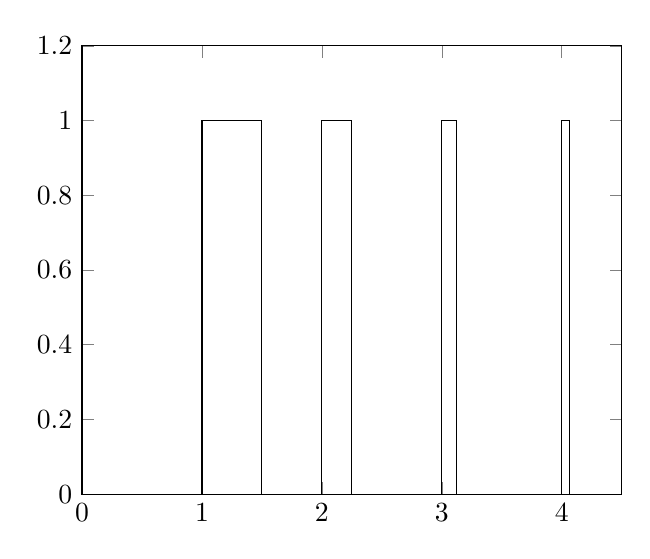
\begin{tikzpicture}
	\begin{axis}[xmin=0, xmax=4.5, ymin=0, ymax=1.2]
		\addplot[samples=20, black] coordinates{(1,0) (1,1) (1.5,1) (1.5,0) (2,0) (2,1) (2.25,1)
			(2.25,0) (3,0) (3,1) (3.125, 1) (3.125, 0) (4,0) (4,1) (4.0625, 1) (4.0625, 0)};	
	\end{axis}
\end{tikzpicture}
\end{figure}
\end{rmk}


\begin{prop}[]
	Let $h: \mathbb{R}_+ \to \mathbb{R}$ be measurable. Assume that $h$ is continuous at a.e. $t \in \mathbb{R}$ and there exists $H$ non-decreasing such that $0 \leq |h| \leq H$ and $\int_{0}^{\infty} H < \infty$. Then $h$ is dRi. 
\end{prop}
\begin{rmk}[]
	In particular if $h$ is bounded, continuous at a.e. $t \in \mathbb{R}$, and vanishes outside a compact set, the $h$ is dRi.
\end{rmk}
{\color{blue}// The proof is omitted and given in Sznitman's notes, I think we should include it here.//}

\begin{theorem}[Smith Key Renewall Theorem]
	Let $h$ be dRi, $F$ non-arithmetic. Then $g=h+h*m$ satisfies 
\begin{align}
\boxed{\lim_{t \to \infty}g(t)= \frac{1}{\mu } \int_{0}^{\infty} h(u) du.}
\end{align}
\end{theorem}

\begin{rmk}[]
	The case $h= \mathbbm{1}_{[0,b]}$ corresponds to the Blackwell Theorem. 
\end{rmk}

{\color{blue}The idea of the proof is to use an approximation of $h$ by functions of the form $h_{c,\Delta}=\sum_{k\geq 0}^{} c_k \mathbbm{1} _{[k\Delta, (k+1)\Delta)}$.}

\begin{proof}
	since $h$ is dRi we have
	\begin{align}
		\sum_{k}^{} \sup_{[k,k+1]}h<\infty.
	\end{align}
	Hence $h(t) \to 0$. Therefore it suffices to prove
	\begin{align}
		\lim_{t\to \infty} \int_{0}^{t} h(t-s)dm(s) = \frac{1}{\mu }\int_{0}^{t} h(u)du.
	\end{align}
	Let $\Delta>0$ such that $F(\Delta) < 1$. 

	Assume $h = \sum_{k\geq 0}^{} c_k \mathbbm{1}_{[k\Delta, (k+1)\Delta)} $ with  $c_k\geq 0$ and $\sum_{k\geq 0}^{} c_k < \infty$. By monotone convergece
	\begin{align}
		h(t-s)dm(s) = \sum_{k\geq 0}^{} \underbrace{c_k [m(t - k\Delta) - m(t-k\Delta - \Delta)]}_{h_{k}(t)}.
	\end{align}
Observe that for every $u\geq \Delta$
 \begin{align}
	 1 \geq F(u) &= m(u) - \int_{0}^{u} F(u-s)dm(s) = \int_{0}^{u} (1-F(u-s))dm(s) \\
		     &\geq \int_{u-\Delta}^{u} (\underbrace{1-F(u-s)}_{\geq1-F(\Delta)}) dm(s) \geq \left(1-F(\Delta)\right)\left(m(u) - m(u-\Delta)\right). 
\end{align}
In the first equality, it was used that $m$ is the solution of the $(F,F)$ renewal equation. Hence for every $t$ and every $k$ 
\begin{align}
	h_k(t) \leq \frac{c_k}{1-F(\Delta)},
\end{align}
by distinguishing between $t-k\Delta \geq \Delta$ and $t-k\Delta<\Delta$, and using that $m$ is non-decreasing, vanishing on $(-\infty, 0)$.
By dominated convergence
\begin{align}
	\lim_{t\to \infty} \sum_{k\geq 0}^{} h_k(t) = \sum_{k\geq 0}^{} \underbrace{\lim_{t\to \infty} h_k(t)}_{\stackrel{\textrm{(Blackwell)}}{=} c_k \frac{\Delta}{\mu }}.
\end{align}
Hence $\lim_{t\to \infty} \int_{0}^{t} h(t-s)dm(s) = \sum_{k=0}^{\infty} c_k \frac{\Delta}{\mu } = \frac{1}{\mu }\int_{0}^{\infty} h(u)du.$ 

Now assume $h\geq 0$ dRi. Let $\Delta>0$ such that $F(\Delta)<1$. Write
\begin{align}
	\underline{h}_{\Delta} &= \sum_{k\geq 0}^{} (\inf_{[k\Delta, (k+1)\Delta]}h) \mathbbm{1}_{[k\Delta, (k+1)\Delta)} \\
	\overline{h}_{\Delta} &=  \sum_{k\geq 0}^{} (\sup_{[k\Delta, (k+1)\Delta]}h) \mathbbm{1}_{[k\Delta, (k+1)\Delta)}. 
\end{align}
We have for every $t$ 
\begin{align}
	\int_{0}^{t} h(t-s)dm(s) \leq \int_{0}^{t} \overline{h}_{\Delta}(t-s) dm(s) \to  \frac{1}{\mu }\int_{0}^{t} \overline{h}_{\Delta}(u)du.
\end{align}
Hence
\begin{align}
	\limsup_{t\to\infty} \int_{0}^{t} h(t-s)dm(s) \leq \frac{1}{\mu }\int_{\mathbb{R}}^{} \overline{h}_{\Delta}(u)du.
\end{align}
Since
\begin{align}
	\left| \int_{\mathbb{R}}^{} \overline{h}_{\Delta}(u) du - \int_{\mathbb{R}}^{} h(u) du \right| \leq \sum_{k\geq 0}^{} \Delta \left(\overline{h}_{\Delta}(k\Delta) - \underline{h}_{\Delta}(k\Delta)\right) \stackrel{\Delta\to0}{\longrightarrow} 0,
\end{align}
where the limit is due to $h$ being dRi. We can let $\Delta$ tend to 0 in the equation above {\color{blue}(with $\limsup$)} to obtain
\begin{align}
	\limsup_{t\to\infty} \int_{0}^{t} h(t-s)dm(s) \leq \frac{1}{\mu }\int_{\mathbb{R}}^{} h(u)du,
\end{align}
and equivalently
\begin{align}
	\liminf_{t\to\infty} \int_{0}^{t} h(t-s)dm(s) \geq \frac{1}{\mu }\int_{\mathbb{R}}^{} h(u)du.
\end{align}
{\color{blue}
\begin{align}
	\frac{1}{\mu }\int_{\mathbb{R}}^{} h(u)du \leq \liminf_{t\to\infty} \int_{0}^{t} h(t-s)dm(s) 
	\leq
	\limsup_{t\to\infty} \int_{0}^{t} h(t-s)dm(s) \leq \frac{1}{\mu }\int_{\mathbb{R}}^{} h(u)du.
\end{align}
}
\end{proof}

{\color{blue}
// This was done in class //

\noindent \textbf{Application} Let $\mu < \infty$. Let $E_t$ be the excess time (time until next renewal) and $e_x(t) = \mathbb{P}_{} \left[ E_t \leq x \right] $. What is $\lim_{t \to \infty} e_x(t)$? We know that $e_x = h_x + e_x*F$, where $h_x(t) = F(t+x)-F(t)$.
\begin{rmk}[]
	$\mu = \mathbb{E}_{} \left[ T_1 \right] = \int_{0}^{\infty} \mathbb{P}_{} \left[ T_1 > t \right] dt$
\end{rmk}
\noindent With this we have that $h_x(t) \leq 1 - F(t) = \mathbb{P}_{} \left[ T_1 > t \right] $, and $1-F(t)$ is non-increasing in $t$ and continuous a.e. (because it is the difference of two monotone functions). 
\begin{align}
	\int_{0}^{\infty} \mathbb{P}_{} \left[ T_1 > t \right] dt = \mathbb{E}_{} \left[ T_1 \right] = \mu < \infty .
\end{align}
Thus (by the proposition) $h_x$ is dRi. Now we can apply the theorem and get that 
\begin{align}
	\lim_{t \to \infty} \mathbb{P}_{} \left[ E_t \leq x \right] = \frac{1}{\mu } \int_{0}^{\infty} h_x(t)dt = \frac{1}{\mu } \int_{0}^{\infty} F(t+x) - F(t) dt,
\end{align}
with $F(t+x) - F(t) = \mathbb{E}_{} \left[ \mathbbm{1}_{T_1 \in (t, t+x]} \right] $, we find that the limit is equal to 
\begin{align}
	\frac{1}{\mu } \int_{0}^{\infty} \mathbb{E}_{} \left[ \mathbbm{1}_{T_1 \in (t, t+x]} \right]dt = \frac{1}{\mu} \mathbb{E}_{} \left[ \int_{0}^{ \infty } \mathbbm{1}_{t \in [T_1 -x, T_1)}    \right]dt = \frac{1}{\mu } \mathbb{E}_{} \left[ \int_{\max\{T_1-x, 0\}}^{T_1} dt \right] =  
	\begin{cases}
		T_1, & T_1 \leq x \\
		x, & T_1 > x.
	\end{cases}
\end{align}
Thus for $t$ large:  $\mathbb{P}_{} \left[ E_t \leq x \right] \approx  \frac{1}{\mu} \mathbb{E}_{} \left[ \min\{T_1, x\} \right]  $. 

\begin{rmk}[]
	$G(x) = \frac{1}{\mu } \mathbb{E}_{} \left[ \min\{T_1, x\} \right] $ is the delay distribution in the proof of Blackwell's Theorem.
\end{rmk}
}
\noindent \textbf{Conclusion} We have now used renewal processes to define a general structure to model a real life process mathematically. Using this object enabled us to implement the LLN and make statements about the asymptotic behavior of such processes over large periods of time.


